%!TEX root = ../Thesis.tex
\chapter{Applications}
\label{chap:applicatons}
In the previous chapters we learned that in addition to viewer's discomfort, reduction of contrast, reduction of stereo acuity, and reduction of overall image aesthetics, crosstalk in stereoscopic screens also has a substantial effect on the observed depth of the disparate objects (i.e., the objects not located at the plane of focus (POF)\index{POF}). The general rule is that the observed depth for any object not lying on the POF will tend to fall back to the POF (losing depth) as the crosstalk level increases, or as the disparity of an object increases. The effect seemed to be more pronounced for objects with narrow width compared to the objects with comparatively wider width, the reason being that the ghost separation (which causes the confusion for HVS) for thin objects is larger for any given disparity. We also learned that, contrary to our intuition, the crosstalk in an automultiscopic screen has little to no effect on the perceived depth for objects of any width for even the most extreme level of crosstalk (14\%). The main reason why crosstalk  did not affect the observed depth might be that in the automultiscopic case, there are two similar ghosts present on each side of the object in both retinal images. This makes the ghost-object combination in both eyes very similar and the HVS might consider them as the same object. Hence, there is nothing to confuse the HVS in estimating the correct disparity between two retinal image patches.

Current literature agree on the theory that the HVS resolves the estimated disparities of objects in a binocular scene by computing the cross-correlation of several patches located at different positions between two perspective retinal images. Finally, we learned that in order to reduce the viewers crosstalk, most of the current state of the art techniques rely upon preprocessing the stereo images in such a way that when, viewed on a stereoscopic or automultiscopic screen, the 
images with system crosstalk added resemble the desired images. Most techniques subtract the pre-calculated light intensity leakage between views from the actual images, and in addition, to using some perceptual measures in order to mask the ghosting that still persists due to the limited dynamic range of the display.

Observed depth reduction due to crosstalk is a serious problem which might alter or degrade the artistic viewing experience for a scene. Similar to image quality metrics e.g., SSIM \cite{wang2004image}, MSE\cite{ wiki:MSE} or VDP\cite{mantiuk2004visible} used to calculate the effects of noise in an image on its perception by a human observer as compared to the noise-free images, it would be useful to have a quality metric that is able to predict the observed depth of objects of interest in a 3D scene based on the crosstalk level of the display along with the dimensions and disparity of the object. Once this prediction is available, the scene artists can then alter the theoretical depths of the objects in order to bring the observed depths as close to the desired depth as possible. For this to work, however, we should have a good understanding of how the HVS estimates the depth from disparity between two retinal images, and hence derive an accurate HVS model. Moreover, reducing the viewer's crosstalk for any given display is also as important if not more for a better viewing experience. The most promising techniques to achieve that use complex optimizations to be performed in order to pre-process the images \cite{van2011perceptually}. It would be helpful if similar effects can be achieved without the mentioned complex and time consuming optimizations.

In this chapter, we will look into a proposed modified HVS depth from disparity resolution model that provides a good initial approximation to the observed depths obtained from our experiment results discussed in the previous chapter. We will also propose two new crosstalk reduction techniques along with their advantages and disadvantages and their results.

\section{Observed depth prediction}

Filippini et al \cite{filippini2009limits} proposed a model that simulated the depth estimation of the HVS via disparity. In short, this model computes the local cross-correlation that is defined by Eq \ref{eq:banks_ccr}.
\begin{equation}
c(\delta_x) = \frac{ \sum\limits_{(x,y) \in W_L} [(L(x,y) - \mu_L)(R(x-\delta_x, y) - \mu_R)] }{\sqrt{\sum\limits_{(x,y) \in W_L}(L(x,y) - \mu_L)^2} \sqrt{\sum\limits_{(x,y) \in W_R}(R(x-\delta_x, y)- \mu_R)^2}},
\label{eq:banks_ccr}
\end{equation}
where
\begin{equation}
W_L \:=\: W_R \:=\: e^{-\left(\frac{x^2}{2\sigma_x^2} \:+\: \frac{y^2}{2\sigma_y^2}\right)}
\label{ccr_windows}
\end{equation}
are anisotropic Gaussian windows (patches) in the left and the right stereo images. The window $W_L$ is fixed in one image while $W_R$ is displaced horizontally while keeping the vertical position constant. For each displacement $\delta_x$, $c(\delta_x)$ is computed resulting in a value in the range [-1,1] (1 if the patches are perfectly correlated, -1 if the patches have no correlation at all). The value of $\delta_x$ for which the maximum cross-correlation is attained is considered to be the disparity of the pixel (centered at the window) in the right image w.r.t the left image. The process is repeated for all the pixels in the left image. The depth estimates using this model, and the human observed depths of the peaks and troughs in random dot stereogram consisting of saw-toothed corrugations of different frequencies and amplitudes were compared by the authors. They found that in addition to their estimated depths matching closely with the viewer's observed depths, their model also correctly estimated the HVS's threshold (for distinguishing between disparities) for the upper and lower spatio-temporal frequencies. However, the random dot stereograms used were devoid of any crosstalk.

We tested the same model on our stimuli (Chapter 4) and found that this model always resulted in the correct disparity of the objects between a stereo image pair. That is, the crosstalk had no effect on the disparity the disparity estimated by the model. This did not match the results we obtained in our experiments with the human observers. The reason is that even though the areas on the images where the ghosts are present will show some positive correlation, the maximum correlation is always obtained at the location where the actual object is located.

Hence it is clear that the HVS does not simply estimate the depth from disparity as the maximum of local cross-correlation only. It is believed that the HVS, while matching patches between retinal images, prefers lower disparity over higher ones \cite{howard1995binocular}. This means that, for any patch in e.g. the left eye retinal image, if the HVS finds two matching patches in the right image, it will choose the one that is closest to the location of the left image patch. Recall from the previous chapter that in the case of stereo displays with some level of crosstalk, for a disparate object in the the left image, the same object is located at some horizontal disparity \emph{d} where as the ghost is located exactly at zero disparity (same location as the location of the object in the left image). Computing a cross-correlation in this case would result in some positive correlation because of the ghost at zero disparity and a highly positive correlation at disparity \emph{d}. To match the results from human observers, the disparity estimator model should have the following characteristics:
\begin{itemize}
\item{Select a disparity \emph{d} based on local cross-correlation.}
\item{In the presence of crosstalk, estimated disparity \emph{d} should shift towards zero disparity gradually as the actual disparity increases over some threshold.}
\item{Estimated disparity should be estimated as 0 if the crosstalk level increases over some threshold (e.g. more than 14\%) or if the disparity is above some level (exceeding Panum's fusion area \footnote{Panum's fusion area is the space around the POF where single binocular vision is observed. Double vision (diplopia) is observed for objects outside the Panum's fusion area.}).}
\end{itemize}
Hence we may assume that the model should somehow weigh the resulting cross-correlation profile prior to obtaining the disparity estimate. We observe that weighing the cross-correlation profile with a Gaussian function centered at the location of ghost in the left eye image fulfills the aforementioned requirements. This can be seen in Fig \ref{fig:windowed_ccr_f}.
\begin{figure}[htbp]
    \centering
    \begin{subfigure}[b]{0.9\textwidth}
        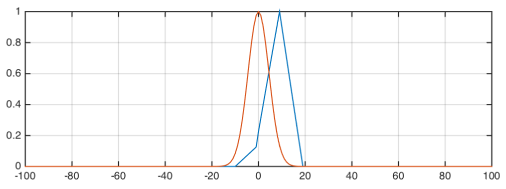
\includegraphics[width=\textwidth]{./Template_Figures/normal_ccr}
        \caption{}\label{fig:normal_ccr}
    \end{subfigure}

    \begin{subfigure}[b]{0.9\textwidth}
        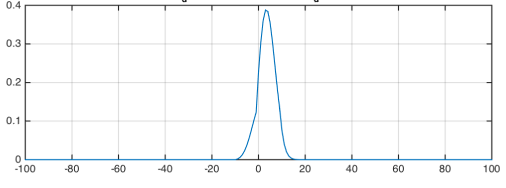
\includegraphics[width=\textwidth]{./Template_Figures/windowed_ccr}
        \caption{}\label{fig:windowed_ccr}
    \end{subfigure}

    \caption{The figure represents estimating the human observed disparity in a thin cylinder stereo pair where the disparity in terms of pixels is 9 and the crosstalk is 14\%. The cross-correlation of a patch containing only the cylinder from the right eye image is computed across the entire left eye image containing both the cylinder and the ghost. (A) The blue line represents the 1D scan line of the result of local cross-correlation. In this case, the maximum cross-correlation occurs at the disparity of 9 pixels, which is the actual disparity. Orange line represents a Gaussian function with $\sigma$ = 9 pixels centered at the location of the ghost that is to be used for weighing the correlation profile. (B) The resulting Gaussian weighted local cross-correlation. It can be seen that, the estimated disparity as a result of the peak of cross-correlation has shifted back from 9 to 3 pixels.\label{fig:windowed_ccr_f}}
\end{figure}

In our disparity estimation model, we assume that the HVS will be able to isolate the object of interest in one (source) retinal image (due to its luminance profile) and try to find an appropriate match for that object in the other target image. The target image has of two possible matches i.e. the ghost and the object itself. For simplicity, we show the resulting cross-correlation for a single scan line of the stereo image pair. This is sufficient to estimate the disparity of a single fixed width object. Figure \ref{fig:normal_ccr} (blue line) represents the cross-correlation profile for a cylinder that has a width of 9 pixels and is located at the disparity of 9 pixel. The background for simplicity in this case is black. We can see that there is some positive correlation at zero disparity due to the 14\% crosstalk induced ghost. However, the full correlation (+1) is attained at the disparity 9, indicating the actual disparity of the object. The orange line represents how the resulting correlation profile is weighted by a truncated Gaussian that has a standard deviation of 9 pixels. The Gaussian weighed correlation profile in Figure \ref{fig:windowed_ccr} is obtained by simple point-wise multiplication of the two functions in Figure \ref{fig:normal_ccr}. It can be seen that after weighing with the Gaussian window for which the standard deviation $\sigma$ is roughly equal to the width of the object, the maximum correlation occurs at a disparity of 3 pixels. This means that, the perceived depth via disparity would be approximately 3 pixels (around 1.18 cm). So, in this, case the estimated disparity is quite close to the result that we obtained from the experiments.

\begin{figure}[H]
\centering
    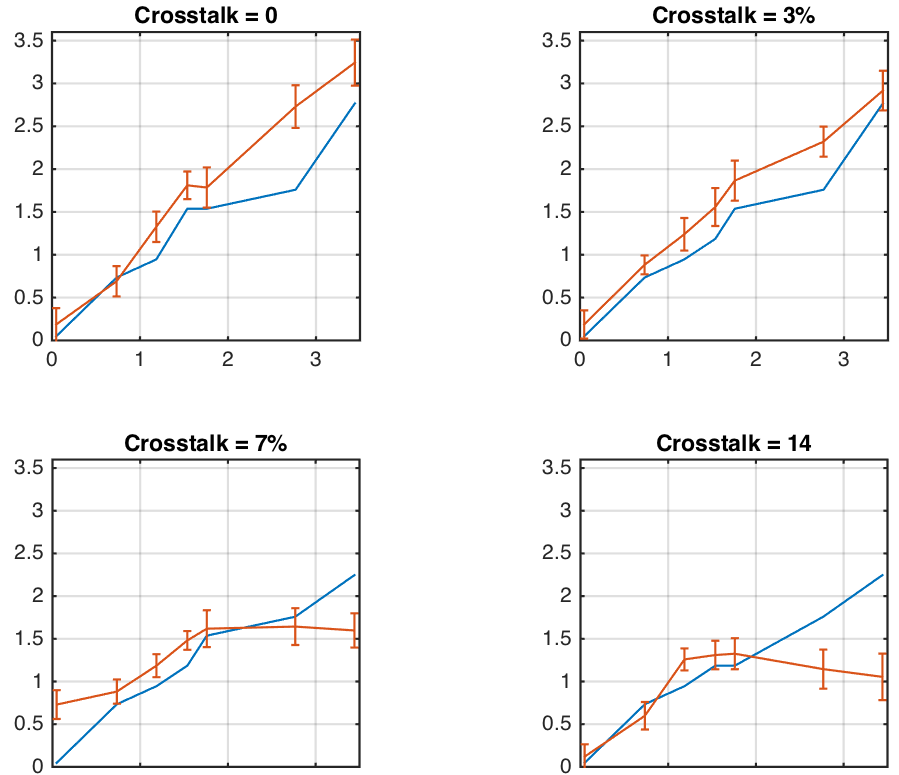
\includegraphics[width=0.7\textwidth]{./Template_Figures/s_9_sigma_7_4}
    \caption{Comparison of experimental observed depth for cylinder of 18.9 arc min width (orange) vs the estimated depth via windowed cross-correlation. The best results were obtained with $\sigma$ = 15.4 arc min.\label{fig:s_9_sigma_7_4}}
\end{figure}
\begin{figure}[H]
\centering
    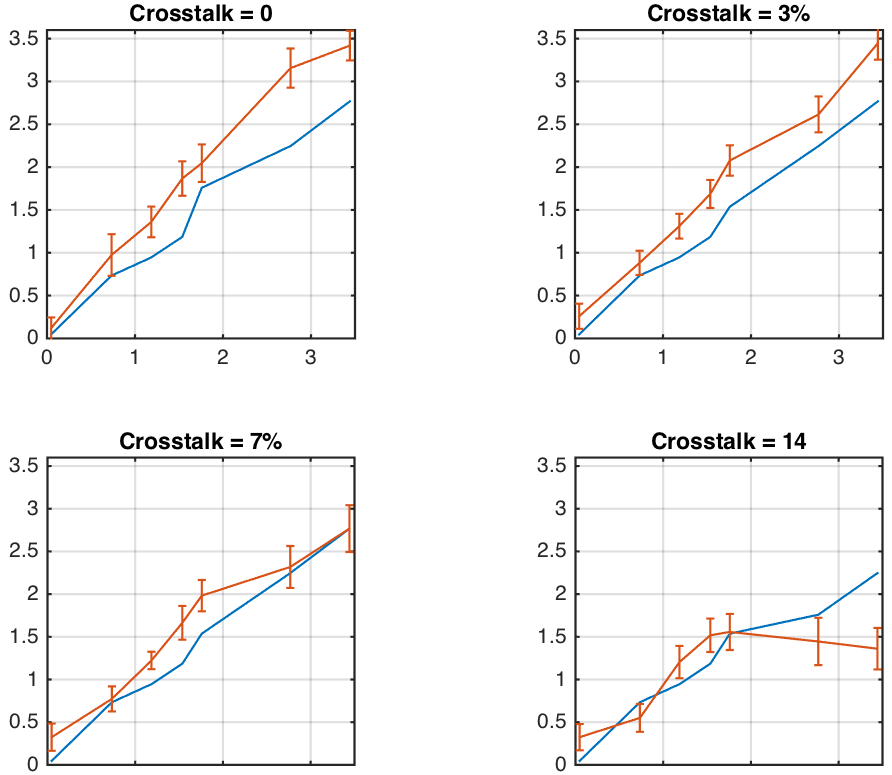
\includegraphics[width=0.7\textwidth]{./Template_Figures/s_18_sigma_14_7}
    \caption{Comparison of experimental observed depth for cylinder of 37.8 arc min width (orange) vs the estimated depth via windowed cross-correlation. The best results were obtained with $\sigma$ = 30.87 arc min.\label{fig:s_18_sigma_14_7}}
\end{figure}
\begin{figure}[H]
\centering
    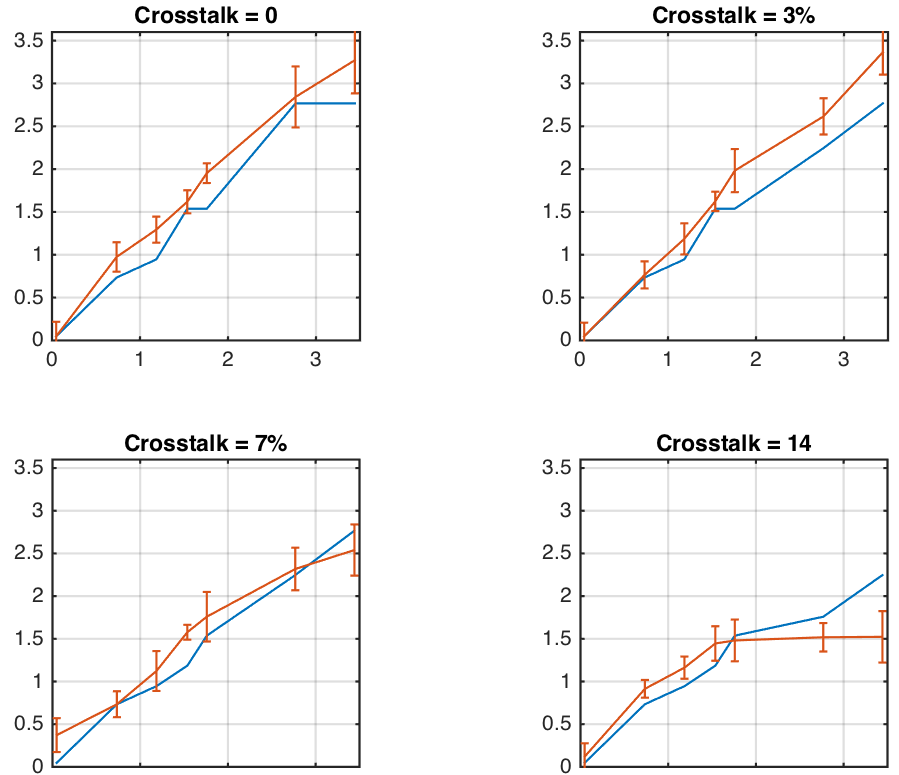
\includegraphics[width=0.7\textwidth]{./Template_Figures/s_27_sigma_17_4}
    \caption{Comparison of experimental observed depth for cylinder of 56.7 arc min width (orange) vs the estimated depth via windowed cross-correlation. The best results were obtained with $\sigma$ = 36.54 arc min.\label{fig:s_27_sigma_17_4}}
\end{figure}
\begin{figure}[H]
\centering
    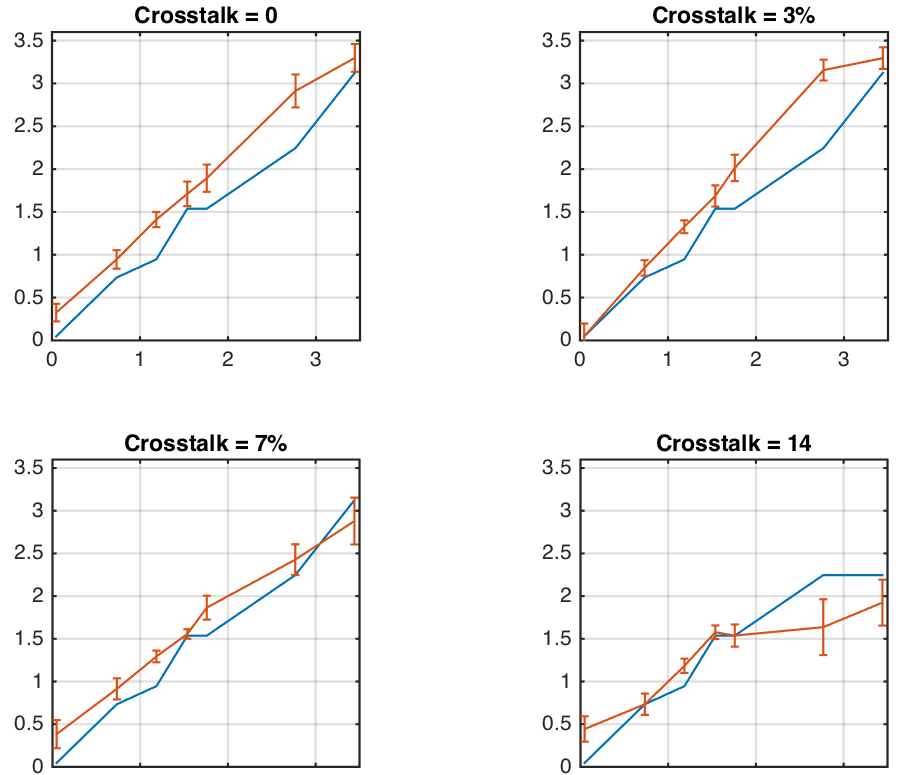
\includegraphics[width=0.7\textwidth]{./Template_Figures/s_36_sigma_22}
    \caption{Comparison of experimental observed depth for cylinder of 75.6 arc min width (orange) vs the estimated depth via windowed cross-correlation. The best results were obtained with $\sigma$ = 46.2 arc min.\label{fig:s_36_sigma_22}}
\end{figure}

\begin{table}[H]
  \begin{center}
    \caption{Coefficient of determination ($r^2$) test results that \textcolor{red}{Change one of the graphs with the new one}}
    \label{tab:model_fitting_test}
    \begin{tabular}{cccccc}
      \toprule
       \specialcell{Stimulus\\width\\(arc min)} &  \specialcell{Comparison\\between\\ }  &  \specialcell{Crosstalk\\level\\(0\%)} & \specialcell{Crosstalk\\level\\(3\%)} & \specialcell{Crosstalk\\level\\(7\%)} & \specialcell{Crosstalk\\level\\(14\%)}\\
      \midrule
      18.9      & BVO & 0.97718     &       0.89288    &    -5.0609   &      -6.0313 \\
                & OVO & 0.78709     &       0.88446    &    -0.25691  &      -0.61822  \\
                & & & & \\
      37.8      & BVO & 0.94688     &       0.96686    &    0.82087   &    -3.2238\\
                & OVO & 0.73072     &       0.80604    &   0.86868    &     0.20619\\
                & & & & \\
      56.7      & BVO & 0.97965     &       0.98846    &    0.70558   &      -2.3817\\
                & OVO & 0.91503     &       0.89967    &    0.89631   &      0.53607\\
                & & & & \\
      75.6      & BVO & 0.95995     &       0.96492    &    0.86452   &      -1.2262\\
                & OVO & 0.85206     &       0.84825    &    0.8946    &      0.50502\\
      \bottomrule
    \end{tabular}
  \end{center}
\end{table}
We simulated our stereo experiments for the cylinders and computed the estimated depths using our Gaussian weighted cross-correlation model. Figures \ref{fig:s_9_sigma_7_4}, \ref{fig:s_18_sigma_14_7}, \ref{fig:s_27_sigma_17_4} and \ref{fig:s_36_sigma_22} show the results that we obtained and there comparison with the data we got from our experiments. We observed that even though this model had some shortcomings and did not fit to all of the data properly, it was able to mimic the degradation of estimated depth as the crosstalk level or the disparity increased. The figures above represent the estimated depths using a our Gaussian weighed local cross-correlation model with fixed $\sigma$ for each cylinder that best matched the data. For almost all the cases (specific disparities and crosstalk levels) where the estimated depth was incorrectly estimated, we were able get approximately matching results using some $\sigma$. However, we were not able to find one $\sigma$ that matched all cases for a particular cylinder. Perhaps the HVS weighs the cross-correlation profile with Gaussians of different standard deviations for different object widths and disparities. Our Gaussian window-weighted local cross-correlation model has the advantage that it resolves to a degraded estimated depth in the case where certain level of crosstalk is present. However, the shortcoming is that it also, to some extent, penalizes the estimated depth even if there is no crosstalk present. This does not conform fully to our experimental data. However, in depth investigation for an HVS depth from disparity model is left as future work.
\pagebreak

\section{Crosstalk mitigation}

During the course of this thesis, we devised and tested some new ideas to improve the current crosstalk reduction techniques. In this section we review those ideas.

\subsection{Unsharp masking in epipolar domain}
The cornsweet illusion \cite{ wiki:cornsweet} is used in contrast boosting image processing techniques such as unsharp masking. The basic idea of unsharp masking is to add to an image a high frequency image of itself. The high frequencies containing image is obtained by subtracting a blurred version of the image from itself. Baar et al\cite{van2011perceptually} used a similar technique to blur the uncorrectable crosstalk in combination with increasing the contrast of the objects around the edges. One can generally use unsharp masking to increase the contrast of an image suffering from contrast loss due to preprocessing for crosstalk compensation . However applying unsharp masking in spatial domain also boosts the unwanted noise. Since automultiscopic screens display light fields, and given the fact that crosstalk in any particular view is induced by the neighboring views, intuitively, it would make sense to apply unsharp masking in the view domain (also called as the epipolar domain) that would result in a crosstalk compensated light field with increased local contrast around the object. Let $\Psi$ be a light field in which x, y denote the spacial dimensions on the displayed image and w denotes the epipolar domain (Figure \ref{fig:lightfeild}).
\begin{figure}[htbp]
    \centering
    \begin{subfigure}[b]{0.48\textwidth}
        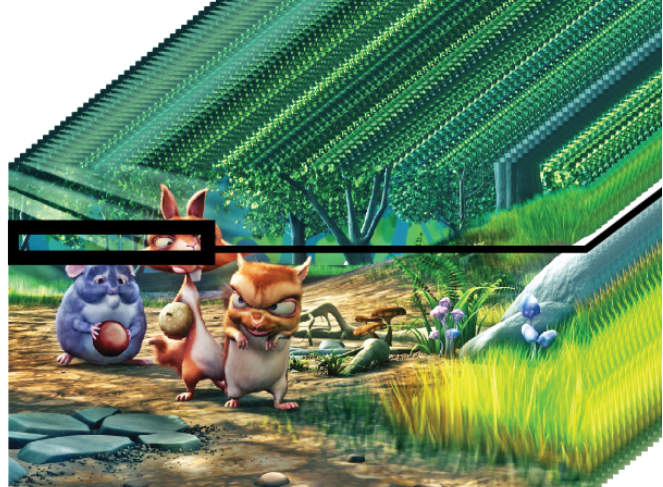
\includegraphics[width=\textwidth]{./Template_Figures/lightfield}
        \caption{}\label{fig:lightfield_rep}
    \end{subfigure}
    \begin{subfigure}[b]{0.48\textwidth}
        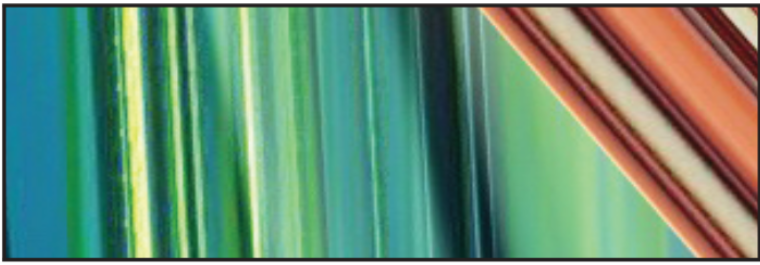
\includegraphics[width=\textwidth]{./Template_Figures/lightfield_epi}
        \caption{}\label{fig:lightfield_epi}
    \end{subfigure}

    \caption{Representation of a 3D light field \cite{du2014improving}. (A)(\emph{x,y}) denotes the view dimensions of a scene to be displayed on an automultiscopic display, whereas \emph{w} denotes different perspective views observed at different viewing locations for the same scene. (B) Epipolar view (\emph{w}) of the 1D scan line in the squared region in (a) representing how every pixels shifts with respect to shift in perspective.\label{fig:lightfeild}}
\end{figure}
\pagebreak

\noindent 
Then for an automultiscopic screen where only the light from the immediate neighbors is leaked, we blur the light field in epipolar domain with the following 1D kernel:
\begin{table}[H]
\centering
\begin{tabular}{|c|c|c|}
\hline
$\omega_1$ & $\omega_2$ & $\omega_3$ \\
\hline
\end{tabular}
\label{tab:blurring_kernel}
\end{table}
\noindent
This will result in an epipolar domain blurred light field $\Psi_{blr}$. Next we subtract $\Psi_{blr}$ from the original light field $\Psi$. This will give us  $\Psi_{hf}$, a light field that only contains luminance-inverted ghosts in every view. i.e.
\begin{equation}
\Psi_{hf}\: =\: \Psi\: -\: \Psi_{blr}
\end{equation}
The crosstalk-compensated light field is obtained as
\begin{equation}
\Psi_{opt}\: =\: \Psi\: +\: \Psi_{hf}
\end{equation}
Hence, for every view image $I \in\: \Psi_{opt}$
\begin{equation}
\begin{aligned}
I_{opt}\: =\:  I + (I - \omega_1I_L - \omega_2I - \omega_3I_R) \\
I_{opt}\: = \: (2-\omega_2)\ I\: -\: \omega_1I_L\: -\: \omega_3I_R
\end{aligned}
\end{equation}
Where $I$ is the view centered image and $I_L, I_R$ are the immediate left and right neighbors respectively. Since the automultiscopic screen will display the optimized light field image as a weighted sum of $I_L, I_R$ and $I$ i.e.
\begin{equation}
\begin{aligned}
I_{observed}\: =\:  \Phi_1.I_{L(opt)}\: + \:\Phi_2.I_{(opt)}\: + \:\Phi_3.I_{R(opt)}       \\
I_{observed}\: = \: \Phi_1{(2-\omega_2) I_L\: -\: \omega_1I_{LL}\: -\: \omega_3I}\:+  \\
                    \Phi_2{(2-\omega_2) I\: -\: \omega_1I_{L}\: -\: \omega_3I_R}\:+   \\
                    \Phi_3{(2-\omega_2) I_R\: -\: \omega_1I\: -\: \omega_3I_{RR}}
\end{aligned}
\end{equation}
Here $I_{LL}$ and $I_{RR}$ are the immediate left and right images to left and right image of the view position in the light field. We know, from view-luminance intensity profiles for an automultiscopic screen \ref{fig:sim_gaussians}, that:
\begin{equation}
\begin{aligned}
\Phi_1\:=\: \Phi_3\:=\: 0.0351,\:\: \Phi_2\:=\:0.8
\end{aligned}
\end{equation}
In order to cancel the effect of $I_L$ and $I_R$ for crosstalk compensation, we choose
\begin{equation}
\begin{aligned}
\omega_1\:=\: \omega_3\:=\: 0.0421,\:\: \omega_2\:=\:1.19
\end{aligned}
\end{equation}
Using the aforementioned values of $\omega_1$, $\omega_2$, $\omega_3$, $\Phi_1$, $\Phi_2$ and $\Phi_3$, the viewer observed image $I_{observed}$ can then be mathematically written as
\begin{equation}
I_{observed}\: =\:  1.42.I\:-\: 0.0014(I_{LL}\:+\:I_{RR})
\label{eq:final_unsharp_obs}
\end{equation}

It can be seen from Equation \ref{eq:final_unsharp_obs} that even though the crosstalk effect induced by the immediate left and right image of a view has been eliminated. However, some over-subtraction of luminance due to the $I_{LL}$ and $I_{RR}$ propagates in the observed image $I_{observed}$. Even though compensating for crosstalk in this manner is quite efficient, one can see the average luminance of the view centered image $I$ has been increased. Since the maximum luminance value an automultiscopic screen can display is 1, our proposed technique will result in clipping of the all the luminance values above 1 hence resulting in loss of contrast. Another drawback is (as described in Figure \ref{fig:why_no_cornsweet}), that unsharp masking in view domain of a light field does not introduce any cornsweet profiles.

\begin{figure}[htbp]
    \centering
    \begin{subfigure}[b]{0.48\textwidth}
        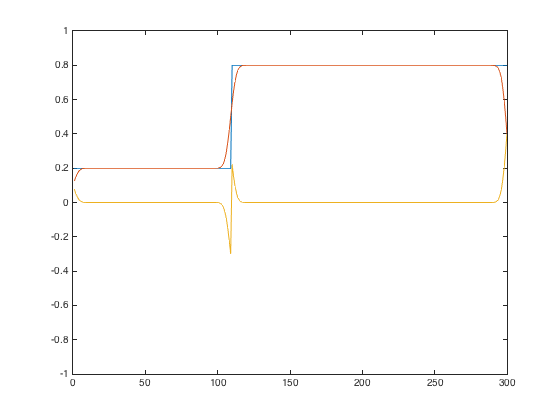
\includegraphics[width=\textwidth]{./Template_Figures/unsharp_proper}
        \caption{}\label{fig:cornsweet}
    \end{subfigure}
    \begin{subfigure}[b]{0.48\textwidth}
        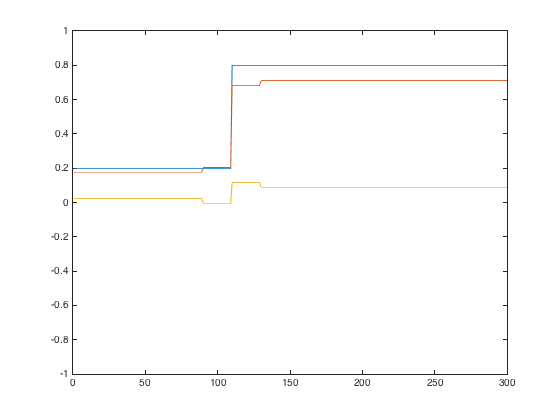
\includegraphics[width=\textwidth]{./Template_Figures/unsharp_epipolar}
        \caption{}\label{fig:no_cornsweet}
    \end{subfigure}

    \caption{(A) 1D representation of luminance profile along an image row. Blue graph represents a luminance step and orange graph represents the luminance profile of the blurred image. Yellow graph represents cornsweet profile centered at the luminance edge and obtained as the difference between the original and the blurred image.  (B) Same procedure performed in view domain. Blue graph represents the luminance profile of a light field image and orange graph represents the non-energy preserving additive blurring due to neighboring views in an automultiscopic environment. The Yellow graph represents the difference between the view image and its view-domain blurred version that resembles closely to subtractive crosstalk cancellation rather than a cornsweet profile.\label{fig:why_no_cornsweet}}
\end{figure}

\subsection{Iterative crosstalk reduction}

To the best of our knowledge, all the current subtractive crosstalk reduction techniques compute the pre-processed crosstalk compensated images by subtracting the amount of leaked light between neighboring views. The calculation of subtracted leaked light is always performed while considering the unmodified stereo image pair. We observe that the amount of light leaked into a view image due to the unmodified alternative view image should be different when the alternate view image is already crosstalk compensated. This, is the case in reality and hence we think that a view image should be compensated appropriately if it's alternative view image is already crosstalk compensated. Inspired by this idea, and the crosstalk cancellation method proposed by \cite{konrad2000cancellation}, we propose an iterative subtractive crosstalk reduction technique for automultiscopic displays.

Consider a light field $\Psi$ consisting of a set of view images ${f_1, f_2, ..., f_N}$. When the $i^{th}$ view is displayed on an automultiscopic screen, its crosstalk $\phi(f_i)$ from the neighboring views can be written as
\begin{equation}
\phi(f_i)\:=\: a_1.f_1\:+\:a_2.f_2\:+\:...\:a_{i-1}.f_{i-1}\:+\:a_{i+1}.f_{i+1}\:+\:...\:a_n.f_n
\end{equation}
Where the light intensity leakage values $a_1...a_n$ are given by the curves in Figure \ref{fig:sim_gaussians}. The crosstalk compensated images $\{\gamma_1...\gamma_n\}$ can then be computed iteratively as:
\begin{equation}
\begin{aligned}
\gamma_1^{n+1} \:=\: f_1 \:-\: \phi(\gamma_1^n) \\
\gamma_2^{n+1} \:=\: f_2 \:-\: \phi(\gamma_2^n) \\
.\:\:\:\:\:\:\:\:\:\:\:\:\:\:\:\:\:\:\:\:\:\:\:\:\:\:\:\:\:\:\:\:\:\:\:\:\:\ \\
.\:\:\:\:\:\:\:\:\:\:\:\:\:\:\:\:\:\:\:\:\:\:\:\:\:\:\:\:\:\:\:\:\:\:\:\:\:\ \\
.\:\:\:\:\:\:\:\:\:\:\:\:\:\:\:\:\:\:\:\:\:\:\:\:\:\:\:\:\:\:\:\:\:\:\:\:\:\ \\
\gamma_N^{n+1} \:=\: f_N \:-\: \phi(\gamma_N^n) \\
\end{aligned}
\end{equation}
Where \emph{n} is the number of current iteration. After each iteration, clipping of the values exceeding the display's dynamic range is performed. The iterations terminate when the error $\epsilon$ falls below a threshold.
\begin{equation}
\begin{aligned}
\epsilon \:=\: \sqrt{(\gamma_1^{n+1}\:-\:\gamma_1^n)^2 \:+\: ...\:+\:(\gamma_N^{n+1}\:-\:\gamma_N^n)^2}
\end{aligned}
\end{equation}

This technique compensates for the crosstalk more appropriately. However, the successive subtraction of luminance from the light field view images between iterations might result in lower average luminance in the crosstalk compensated light field (Figure \ref{fig:iterative_tech}).
\begin{figure}[htbp]
    \centering
    \begin{subfigure}[b]{0.48\textwidth}
        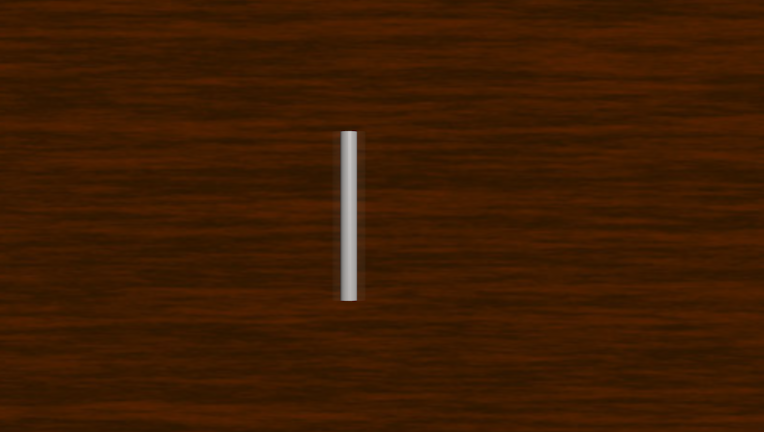
\includegraphics[width=\textwidth]{./Template_Figures/image_w_ct}
        \caption{}\label{fig:original_lf}
    \end{subfigure}

    \begin{subfigure}[b]{0.48\textwidth}
        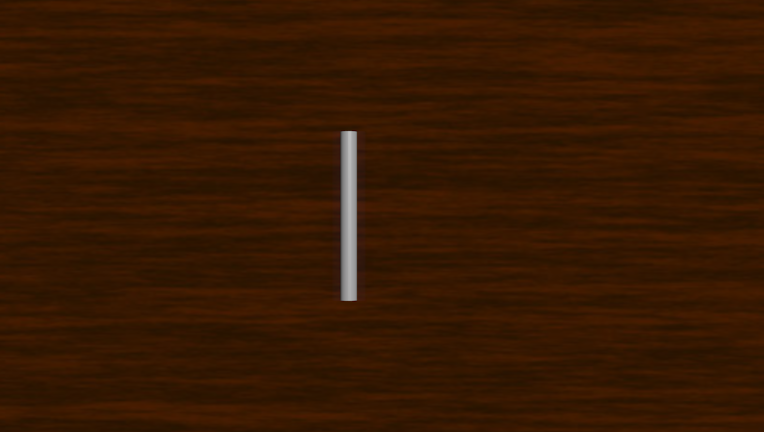
\includegraphics[width=\textwidth]{./Template_Figures/subtractive_comp}
        \caption{}\label{fig:subtractive_lf}
    \end{subfigure}
    \begin{subfigure}[b]{0.48\textwidth}
        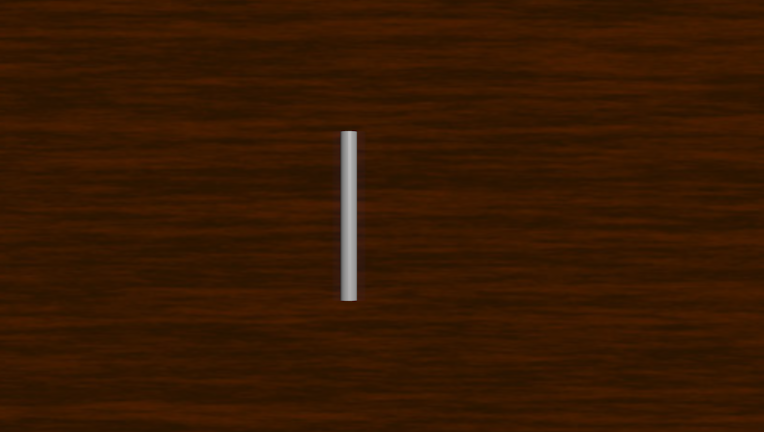
\includegraphics[width=\textwidth]{./Template_Figures/iterative_comp}
        \caption{}\label{fig:iterative_lf}
    \end{subfigure}

    \caption{Naive subtractive crosstalk compensation compared to our proposed iterative crosstalk compensation. Due to the fact that ghosting is not visible in the figure on printed document, viewers are encouraged to view this document in electronic form. (A) A displayed view image for automultiscopic display containing crosstalk given by the curves in Figure \ref{fig:sim_gaussians}. (B) Displayed compensated view image using naive crosstalk subtraction. (C) Displayed compensated view image using our iterative crosstalk subtraction. \label{fig:iterative_tech}}
\end{figure}


% \subsection{Proposed optimizations}
% \subsection{Unsharp masking in view domain}
% \subsection{Iterative subtraction}
